\chapter{はじめに}
\thispagestyle{myheadings}

% **DIOCOMO2019 ========================================================**
\section{研究背景}
コロナウイルスの流行によって巣ごもり需要が拡大し,Netflixや YouTube,ニコニコ動画といった動画共有サイトの利用が広がっている.これらのサービスはテレビ番組とは異なり,ユーザの好きな時間に好きなコンテンツを選択して視聴できるため,自分の好みやライフスタイルに合わせて映像コンテンツを楽しめる.動画共有サイトなどに投稿された映像コンテンツは,利用の手軽さからスマートフォンを通して視聴される場合が多いが,その利点と引き換えにコンテンツが本来持っている視聴体験が失われる場合がある.例えば映画館で上映される映像コンテンツは,大きなスクリーンと高音質なオーディオシステムを用いて投影されるのを前提として制作されている.そのため,映画館以外で視聴した場合には本来の映像美や迫力が減少してしまう.特に,3Dや4DXで上映される映像コンテンツは,物理的/性能的な問題から自宅でのPCでは視聴体験を再現するのは不可能である.

動画プラットフォームとして,ニコニコ動画,YouTube,Netflix,Amazon Prime Video,Huluなどがあり,多様なジャンルの動画を提供しており,好みに合わせたコンテンツを視聴することができます.

ニコニコ動画は,動画視聴している際に視聴者が動画の任意の再生時間に対して,コメントの投稿ができる.生配信のコメントは視聴している人が同時視聴している他人のコメントを見れる,同時視聴者との会話や盛り上がっている瞬間を文字として共有が可能である.コメントは,他ユーザに表示され動画へのリアルタイム共有される.表示されるコメントは,文字のスタイルや大きさ,色といった調節ができる.絵文字や記号や文字を組み合わせた視覚的表現をアスキーアートと呼ぶ.
視聴体験を増幅するために,コメントの投稿による感情の共有やアスキーアートを用いた.動画への表示は,コンテンツ自体にない楽しさを引き出す面白い手法といえる.しかし,ニコニコ動画のコメントは動画自体に重量されるものであり,動画コンテンツを視聴する際に見づらい場合があるといえる.その例を図に示す.
\begin{figure}[H]
    \centering
    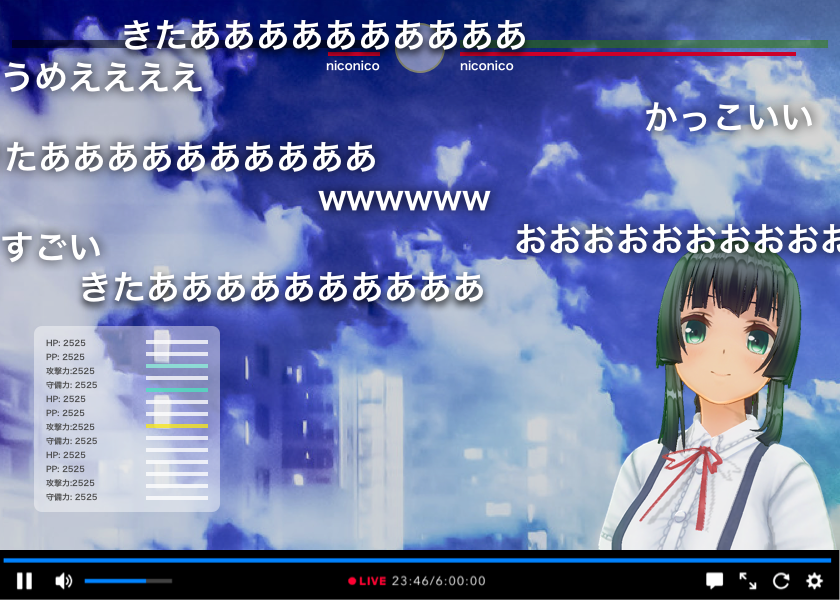
\includegraphics[width=10cm]{images/chapter1/nikoniko_grafu.png}
    \caption{視聴体験を向上させるサービス例 (ニコニコ動画の流れるコメント)}
\end{figure}

YouTubeは,動画の中で最も視聴された部分を示すグラフ,プログレスバー(再生バー)の上部に表示される.視聴数が多い箇所は山が高い山になって表示され,ユーザーによって多く再生された箇所であることを示す.
最も視聴数を集めた箇所のサムネイルには,「リプレイ回数が最も多い部分」と表示されるので視認性も高める効果がある.グラフは常時表示されるわけではなく,プログレスバーの赤いポインタで動画をスキップしているときに表示される.グラフ機能の導入により,ユーザーは長尺の動画でもグラフを見れば「重要なポイント」「見た方が良い箇所」というのが、ひと目で把握することができる.プログレスバーのグラフ表示は,Web版YouTubeとモバイルアプリ版YouTubeの両方に提供されている.再生画面上だけで操作・確認ができるので、コメント欄を確認する手間も省かれる.その例を図に示す.
\begin{figure}[H]
    \centering
    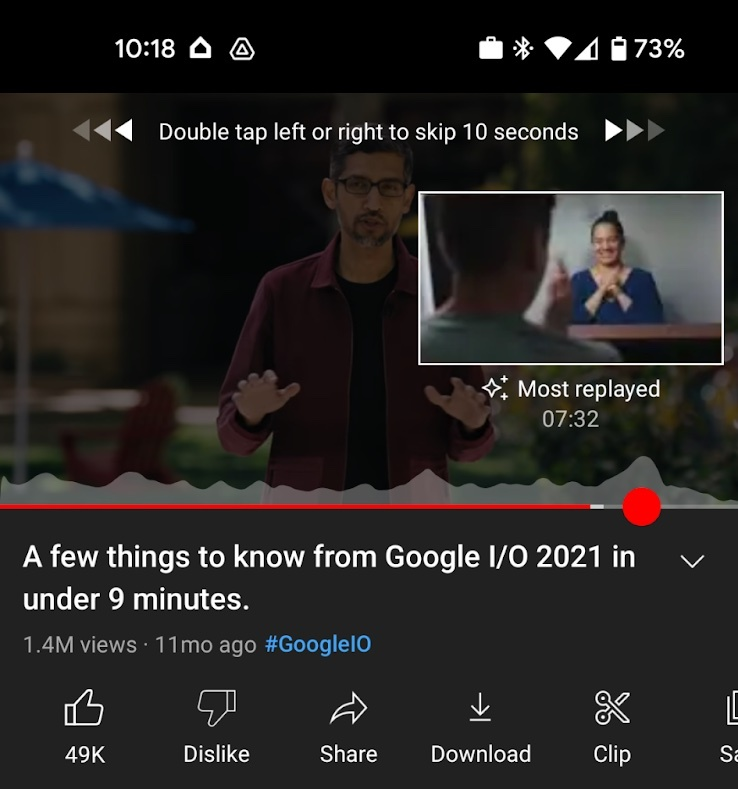
\includegraphics[width=10cm]{images/chapter1/YouTube.jpeg}
    \caption{視聴体験を向上させるサービス例 (Youtubeの最も視聴された部分を示すグラフ)}
\end{figure}

人間の視野には中心視野と周辺視野と呼ばれる部分が存在する.中心視は視線を合わせた物をはっきりと認識する能力,周辺視は物をぼんやりとしか知覚できない代わりに全体像を瞬間的に知覚する能力である.ここで,周辺視は中心と比べて,一度に得られる情報が多く,目に入った情報の処理も無意識的に行われるので目の疲労度も少ないなどの利点がある.また,ホラー映画などのコンテンツは周辺視を利用してより視聴者の恐怖を高めるなどの手法をとっている.周辺視を効果的に使うことで動画の面白さを増幅できると考えられる.

技術的背景として,ニコニコ動画のコメントをリアルタイムに表示するには,ネットワークや通信プロトコルの進歩,動画配信は大容量の動画データをストリーミングできる環境の進歩によって実現可能になった.
ネットワークや通信プロトコルの進歩は,LTE(ロングタームエボリューション)などの高速ネットワークの展開と,スマートフォンや様々なクラウドサービスの普及により,インターネットを流れるデータ量は急激に増大している.スマートフォンやパソコンを用いて,日常的に様々なインターネットサービスを利用しています。新たなスマートデバイスやIoT(Internet of Things)サービスの普及,5G(第五世代移動通信システム)の商用展開などに従い,暮らしを支えていく上で,インターネットへの接続はますます欠かせないものとなっていくといえる.そして,インターネットにおいて広く利用されているのがTCP/IP(Transmission Control Protocol/Internet Protocol)と呼ばれるプロトコルです.
TCP/IPは1980年頃に基本形が完成以来,インターネットの普及とともに拡大し,発展を続けてきました.TCP/IPが普及した要因の一つとして,ネットワークの機能を必要最小限に低減するというコンセプトが挙げられる.ネットワークを高機能化すると,一般的にコストが高くなる,相互接続が難しくなる,構築や保守が困難になる,といった弊害が発生する.問題を避け,シンプルなネットワークを指向したことが,TCP/IPの特長であると言える.しかし,時代の推移に従い利用されるアプリケーションや通信環境が変化するに従って,これらのプロトコルにも様々な改良が重ねられている.

大容量の動画データをストリーミングできる環境の進歩は,高速なブロードバンド環境が整備され,ストリーミング配信の定額制サービスが急速に普及しています.
ストリーミングとは,インターネットを介した動画配信や音楽配信に用いられる配信方式で、「オンデマンド型」と「ライブ型」の2種類がある。データのダウンロード後に視聴を開始するのではなく,データを受信しながら同時に随時再生していくという点がストリーミング方式の特徴である.従来はCDやDVDといった記録媒体に保存されたデータを読み込む、あるいはインターネット経由でデータのダウンロード完了後にファイルを再生する方式が一般的である.
ファイルサーバーやクラウドストレージでの共有,またはWebサーバーを使ったダウンロード配信は,ファイルの流失および不正な持ち出しといったセキュリティリスクが懸念されている.そのため,機密情報を含む動画コンテンツの共有に適しているとは言い難いのが現状である.企業が動画コンテンツを活用する場合はセキュリティ面を考慮する必要があるため,動画配信サービスを使ったストリーミング配信が最も適しているといえる.
動画配信サービスを使ったストリーミング配信であれば,さまざまなデバイスに柔軟に対応できると同時にファイルが端末に残らない.機密情報の漏洩や意図的な流出といったセキュリティリスクを最小限に抑えられる.ID認証やパスワード認証,またはIPアドレス制限やアクセス権限などを細かく設定することでセキュアな配信環境を整備できるのも大きなメリットであるといえる.	


% **DIOCOMO2020 (ryoga)====================================================**
\section{目的とアプローチ}
本研究の目的は,自宅での動画視聴に迫力を加えるコンテンツの開発である.
既存のコンテンツは,気軽に自宅や外出時のスマートフォンで,コンテンツを視聴できるようになっている.しかし,現在のコンテンツでは映像体験を得ることは難しいといえる.これらを解決するには,コンテンツに対してさらなる楽しみ方を提供する.つまりコロナ禍において自宅で過ごす時間が増え、新たにコンテンツに対してさらなる楽しみ方を提供する必要がある。そういった問題を包括的に解決するために、コンテンツを視聴しているときの生体データを使用し,盛り上がりがあるシーンに迫力を加える.つまりコンテンツ視聴時の生体データを集め,取得したデータを基に迫力を加えるコンテンツを開発する.生体データを使用とは、コンテンツを視聴している時の生体データを取得することで感情を抜き出し,そのコンテンツにおいて盛り上がりの部分を推定する.盛り上がりがあるシーンに迫力を加えるとは、盛り上がりの部分が抜き出された情報を使いコンテンツに効果を加える.効果を加えるとは,エフェクトを画面全体に重畳表示し視聴している動画に対して,より興奮した/緊迫感を得た,という結果が得られる.

\section{論文構成}
本稿の構成は以下の通りである.2章では本研究に関連する研究として生体データする研究,重畳提示に関する研究を紹介する.3章ではコンテンツ視聴時に生体データを取得しコンテンツへ重畳提示手法についての提案を行う.第4章では評価実験を行い、本稿で提案した手法について生体データと重畳提示の二つに分けて評価する.5章ではまとめと今後の課題を述べる.

